\section{Úchovávání dat}
Jak již bylo zmíněno, uživatelská data a samotná aplikace musí být někde uchovávány. Webová aplikace (tj. VueJS frontend a Laravel backend) je nasazena pomocí služby "App Platform" od poskytovatele DigitalOcean. PostgreSQL databáze pro administraci nad uživatelskými daty a formuláři, jejíž struktura bude rozebrána v této části, je nasazena na Heroku serveru. 

	\subsection{Struktura databáze}
	K tomu, aby byla struktura databáze vysvětlena, je níže vygenerováno schéma pomocí programu DataGrip !!!citace!!!, které by mělo sloužit pro lepší vizualizaci.
	
	\begin{figure}[h]
		\centering %% příkaz, který ti obrázek zarovná na střed
		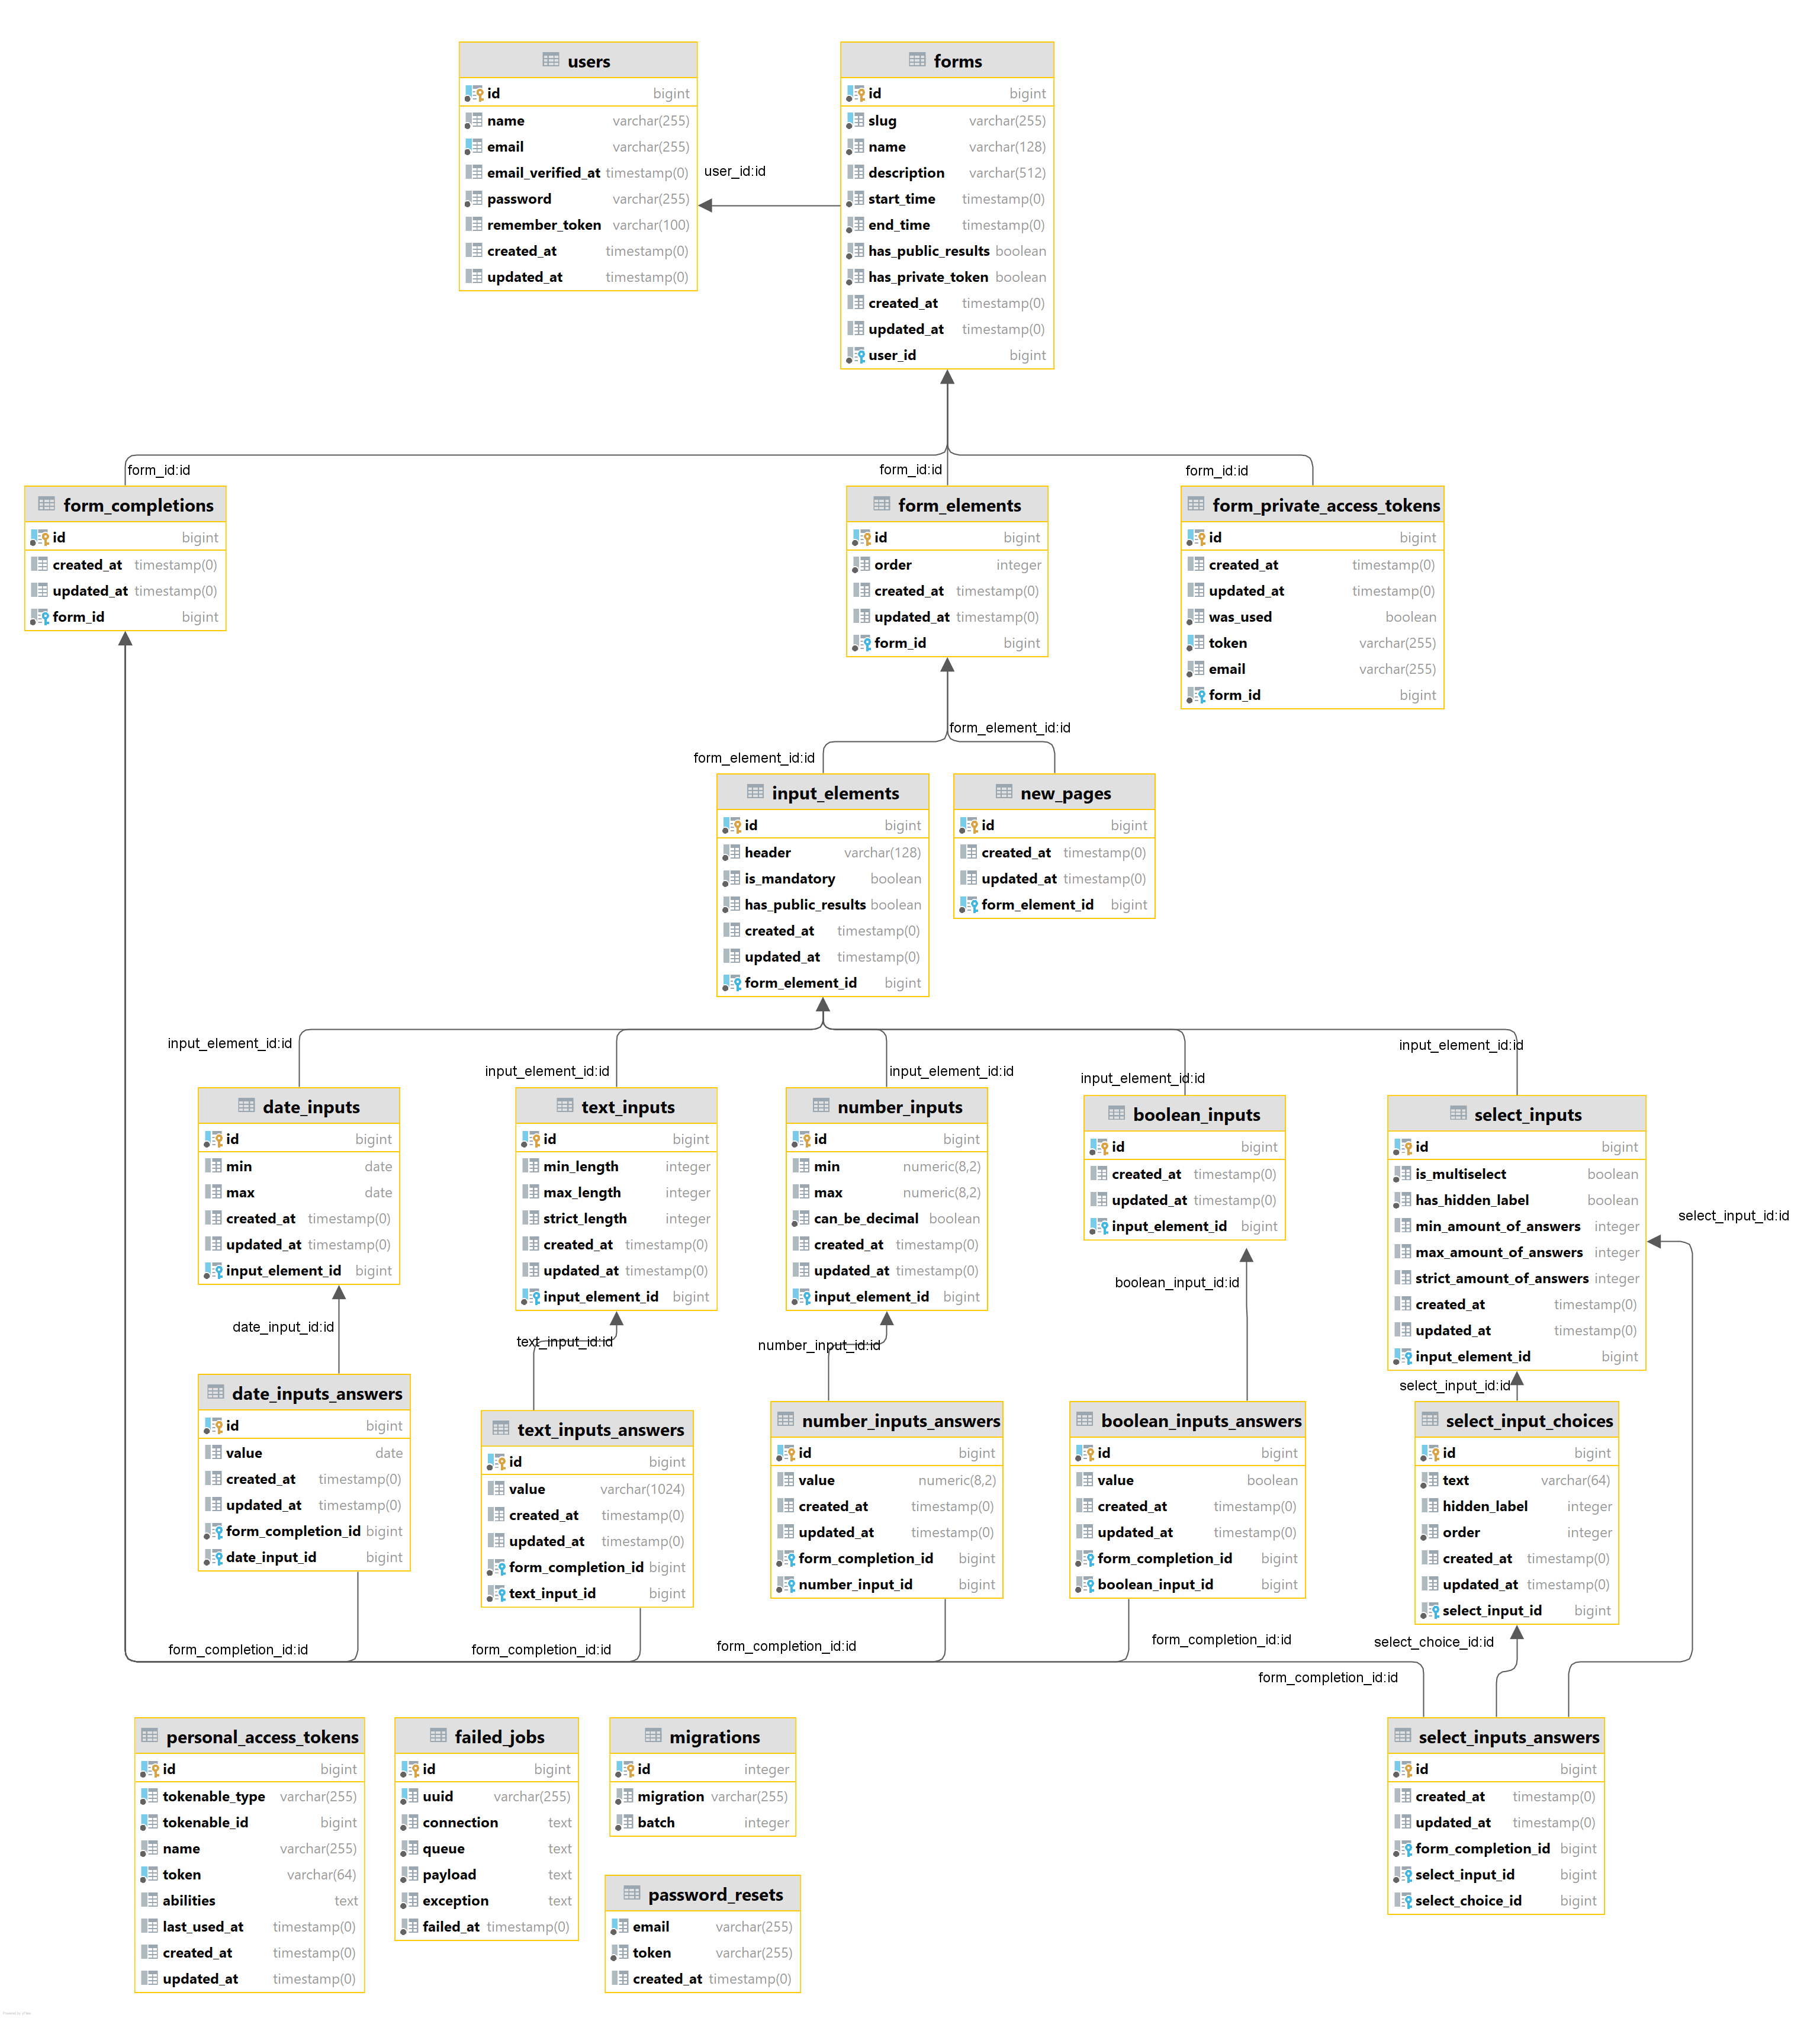
\includegraphics[width=0.65\textwidth]{img/db_diagram.png} %% vložení samotného obrátku
		\caption{Diagram struktury databáze} %% popisek obrázku, nezapomeň na citace!
		\label{fig:db_diagram} %% označení až budeš chtít na obrázek odkazovat
	\end{figure}
	
	Jak je již z obrázku vidět, databáze je tvořena tabulkami, které jsou provázány určitými relacemi. Všechny tabulky (kromě tabulky \textit{password\_resets} atribut \textit{id}) mají unikátní primární klíč, kterým lze identifikovat jednotlivé instance. Většina z nich má také tzv. cizí klíč, který slouží k propojení s jinou tabulkou na základě shody tohoto klíče s cizím primárním klíčem. Také většina obsahuje předgenerované atributy timestamps (v překladu časová razítka) \textit{created\_at} a \textit{updated\_at}, které nám umožňují sledovat, kdy byla položka vytvořena či upravena.
	
	V práci nebudou popsány tabulky \textit{personal\_access\_tokens}, \textit{failed\_jobs}, \textit{migrations} a \textit{password\_resets}, jelikož se jedná o předgenerované tabulky Laravelem. Výjimkou je tabulka \textit{users}, která byla cíleně využita.
	
	\subsubsection{Uživatelé}
	Základním objektem databáze je samotný uživatel (tabulka \textit{users}), který obsahuje standardní vlastnosti jako jsou: uživatelské jméno (\textit{name}), emailovou adresu (\textit{email}), která také slouží jako identifikátor (musí být unikátní), heslo v zašifrované podobě (\textit{password}) a další předgenerované atributy, které jsou využívány primárně samotným frameworkem Laravel. V rámci relací pro uživatele platí, že může mít více formulářů.
	
	\subsubsection{Formuláře}
	Dalším důležitým základním objektem je formulář (tabulka \textit{forms}). Tento objekt reprezentuje samotný dotazník a jeho vlastnosti. Základním atributem je unikátní řetězec (\textit{slug}), který má podobnou funkci jako primární klíč - ukazuje na konkrétní formulář. Dalšími atributy jsou: název formuláře (\textit{name}), nepovinný popis formuláře (\textit{description}), čas zveřejnění a čas ukončení zveřejňování (\textit{start\_time} a \textit{end\_time}), proměnná vyjadřující dostupnost formuláře - zda je veřejný nebo privátní s nutností vyplnění přes pozvánku (\textit{has\_public\_results}) a proměnná ukazující, zda má formulář veřejně dostupné výsledky (\textit{has\_public\_results}). Tento objekt je vázán na další databázové objekty těmito vztahy: formulář musí mít jednoho uživatele (vlastníka) a musí mu náležet přístupové tokeny v případě privátního formuláře (tabulka \textit{form\_private\_access\_tokens}), samotné elementy formuláře (tabulka \textit{form\_elements}) a záznamy vyplnění formuláře (tabulka \textit{form\_completions}).
	
	\subsubsection{Elementy formuláře}
	Podstatným prvkem po objektu samotného formuláře jsou tzv. elementy formuláře (tabulka \textit{form\_elements}) - ty zaobalují další meziprvky jako jsou element pro uživatelský vstup (tabulka \textit{input\_elements}) a element pro označení nové stránky (tabulka \textit{new\_pages}) a přiřazují jim pořadí (atribut \textit{order}), jak se mají ve formuláři zobrazovat. Tento prvek vznikl právě pro sjednocení hodnoty pořadí. Platí pro něj vztah, že mu musí náležet buď element pro uživatelský vstup nebo element označující novou stránku. Zároveň, jak již bylo zmíněno, sám musí náležet samotnému formuláři.
	
	Jedním ze zmíněných meziprvků elementu formuláře je element označující novou stránku (tabulka \textit{new\_pages}). Jeho využití je prosté - odděluje od sebe elementy pro uživatelský vstup, což při vykreslování formuláře slouží ke stránkování. Má jedinou vazbu - musí náležet elementu formuláře (tabulka \textit{form\_elements}).
	
	Dále přichází na řadu objekt elementu pro uživatelský vstup (tabulka \textit{input\_elements}), jehož účelem je hlavně zaobalení jednotlivých typů uživatelských vstupů. Také ale obsahuje atributy jako samotnou otázku (\textit{header}), proměnnou popisující, zda musí být otázka povinně vyplněna (\textit{is\_mandatory}) a proměnnou ukazující, zda jsou veřejně publikovány výsledky zodpovězení příslušné otázky (\textit{has\_public\_results}). Kromě vazby, že jako element nové stránky náleží elementu formuláře, tak mu musí náležet příslušný objekt typu vstupu (např. tabulka \textit{text\_inputs}).
	
	\subsubsection{Typy vstupů}
	Dalšími prvky, které zde budou rozebrány, jsou právě objekty typu vstupu. Těchto typů existuje v databázovém modelu několik:
	
	\begin{itemize}
		\item \textbf{Textový vstup} (tabulka \textit{text\_inputs}) - typ zaznamenávající textovou odpověď, kterému lze přiřadit validační atributy jako minimální, maximální či striktní délku (\textit{min\_length}, \textit{max\_length}, \textit{strict\_length}).
		\item \textbf{Číselný vstup} (tabulka \textit{number\_inputs}) - typ zaznamenávající odpověď ve formě čísla, kterému lze nastavit validační atributy jako minimální a maximální hodnota (\textit{min} a \textit{max}) či zda může být zadaná hodnota desetinné číslo (\textit{can\_be\_decimal})
		\item \textbf{Vstup pro datum} (tabulka \textit{date\_inputs}) - typ pro zaznamenávání odpovědí ve formě data, kterému lze přiřadit validační parametry jako minimální a maximální datum (\textit{min} a \textit{max})
		\item \textbf{Vstup pro odpověď typu Ano/Ne} (tabulka \textit{boolean\_inputs})
		\item \textbf{Vstup pro odpověď z výběru předepsaných možných odpovědí} (tabulka \textit{select\_inputs}) - typ zaznamenávající, jakou odpověď (pocházející z tabulky \textit{select\_input\_choices}) dotyčný respondent pro příslušnou otázku vybral; lze u něj validovat zda se jedná o tzv. multiselect (možnost výběru více odpovědí - v tomto případě lze omezit i minimální, maximální nebo striktní počet odpovědí pomocí atributů \textit{min\textbackslash max\textbackslash strict\_amount\_of\_answers}) či singleselect (možnost zvolení pouze jedné odpovědi) podle atributu \textit{is\_multiselect} a zda má skrytý popisek používaný pro export dat podle atributu \textit{has\_hidden\_label}
	\end{itemize}
	
	V rámci vztahů pro všechny platí, že jsou podřízení elementu pro uživatelský vstup. Dále platí, že každému jednotlivému typu vstupu náleží tabulka pro zaznamenávání odpovědi (např. tabulka \textit{number\_input\_answers}).
	
	Speciálním případem je poslední zmíněný vstup pro odpověď z výběru předepsaných možných odpovědí. K němu je vytvořena tabulka \textit{select\_input\_choices}, sloužící k ukládání jednotlivých možností odpovědí k nadřazenému vstupu pro odpověď. Jsou zde obsaženy tyto atributy: text vyjadřující možnou odpověď (\textit{text}), skrytý popisek pro export (\textit{hidden\_label}) a pořadí, jak mají být možnosti otázky seřazeny.
	
	\subsubsection{Odpovědi k otázkám}
	Dalšími objekty jsou odpovědi k otázkám, které - jak už z jejich názvu vyplývá - slouží k zaznamenávání příslušných odpovědí k jednotlivým otázkám. Je jich stejné množství jako počet typů vstupů a s každým tímto vstupem jsou samozřejmě relačně provázány - musí náležet jak příslušnému typu vstupu, tak i objektu vyplnění formuláře (tabulka \textit{form\_completions}). Obsahuji kromě standardních atributů jen atribut hodnoty (\textit{value}), ve kterém je uložena právě odpověď na otázku.
	
	Jedinou výjimkou je znovu objekt pro zaznamenávání odpovědí pro otázky s výběrem předepsaných možných odpovědí. V něm není hodnota uložena ve sloupci \textit{value}, ale jako cizí klíč odkazující na příslušnou možnost otázky.
	
	\subsubsection{Vyplnění formuláře}
	Dalším objektem, který je nutné evidovat, je záznam o vyplnění nebo-li odeslání odpovědí formuláře (tabulka \textit{form\_completions}). Ten seskupuje odpovědi z jednotlivých otázek ve formuláři pro jednu odpověď. Je přímo vázán se samotným formulářem, kterému musí vždy patřit a musí mu náležet jednotlivé odpovědi k otázkám.
	
	
	